\subsubsection{Generative Adversarial Imitation Learning}
\label{sec:gail}
The \textit{Generative Adversarial Imitation Learning} (GAIL) is a Learning from Demonstration approach proposed by the authors of \cite{ho2016gail}. The rationale behind GAIL was to improve the Inverse Reinforcement Learning (IRL) setting, which is expensive to run due to the double-nested optimization procedure. To achieve this objective, the authors in \cite{ho2016gail} started from the Max-Ent formulation in Formula \ref{formula:regularized_max_ent}, and obtained a characterization of the learned policy. This characterization combines the learning of the reward function and the learning of the policy through a reinforcement learning algorithm. In Formula \ref{formula:regularized_max_ent}, $\psi(c)$ is a cost-regularizer, $\psi^{*}(c)$ is its conjugate, and $\rho_{\pi}$ is the occupancy measure, i.e., the distribution of state-action pairs that the agent encounters when navigating the environment with policy $\pi$. 

The next step was to choose an appropriate regularization function. In particular, by choosing the regularizer in Formula \ref{formula:ga_regularization}, the conjugate in Formula \ref{formula:ga_regularizer_conjugate} can be obtained. This is the classic Adversarial Learning Loss, where the current policy $\pi^{L}$ acts as the GAN generator, and $D$ is the GAN discriminator, which must distinguish between state-action pairs generated either by the expert policy or by the current policy.

\begin{equation}
    \label{formula:regularized_max_ent}
    \begin{aligned}
        IRL_{\psi}(\pi^{E}) = \underset{c \in \mathbb{R}^{S \times A}}{\operatorname{arg\,max}} &  - \psi(c) +  \\
        & \left(\underset{\pi^{L} \in \Pi}{\min} -\mathcal{H}(\pi^{L}) + \mathbb{E}_{\pi^{L}} \left [ c(s,a) \right ]\right) - \\
        &  \mathbb{E}_{\pi^{E}} \left [ c(s,a) \right ]
    \end{aligned}
\end{equation}

\begin{equation}
    \label{formula:policy_characterization}
    \begin{aligned}
    RL \circ IRL_{\psi}(\pi^{E}) = \underset{\pi^{L} \in \Pi}{arg \ min}-\mathcal{H}(\pi^{L}) + \psi^{*}(\rho_{\pi^{L}} - \rho_{\pi^{E}}) 
    \end{aligned}
\end{equation}

\begin{equation}
    \label{formula:ga_regularization}
    \begin{split}
    \psi_{GA}(c) = \left\{
    \begin{matrix}
        \mathbb{E}_{\pi^{E}}\left[ g(c(s,a)) \right] & \text{if } c < 0\\ 
        +\infty & \text{otherwise}
    \end{matrix}
    \right.,
    \\
    g(x) = \left\{
    \begin{matrix}
        -x - \log(1- e^{x}) & \text{if } c < 0\\ 
        +\infty & \text{otherwise}
    \end{matrix}
    \right.
    \end{split}
\end{equation}

\begin{equation}
    \begin{aligned}
    \label{formula:ga_regularizer_conjugate}
    \psi^{*}_{GA}(\rho_{\pi^{L}} - \rho_{\pi^{E}}) = \underset{D\in(0,1)^{S \times A}}{max} \mathbb{E}_{\pi^{L}}\left [ \log(D(s,a))\right ] + & \\ \mathbb{E}_{\pi^{E}}\left [ \log(1 - D(s,a))\right ]
\end{aligned}
\end{equation}
Based on these considerations, Algorithm \ref{alg:gail} has been proposed. Specifically, the GAIL algorithm is an iterative procedure composed of two main steps. The first step involves updating the discriminator $D$, which must distinguish between trajectories produced by the learned policy $\tau^{L}_{i}$ and trajectories produced by the expert $\tau^{E}$. The second step involves updating the learner policy $\pi^{L}$ according to some reinforcement learning algorithm (e.g., TRPO was used in \cite{ho2016gail}). The policy is updated in such a way that the trajectories it generates become indistinguishable from those of the expert for the discriminator, i.e., the learner produces state transitions that are similar to those of the expert.
\begin{algorithm}[tb]
\caption{Generative Adversarial Imitation Learning Algorithm}\label{alg:gail}
\begin{algorithmic}
\Require Expert Trajectories $\tau^{E} \sim \pi^{E}$, initial policy $\pi^{L}_{\theta}$, discriminator $D_{\omega}$
\For {$i=1, \dots, N$} 
    \State Sample trajectories, $\tau^{L}_{i} \sim \pi^{L}_{\theta}$
    \State Update Discriminator, $\mathbb{\hat{E}}_{\tau^{L}_{i}}\left [\nabla_{\omega} \log(D_{\omega}(s,a))\right ] +\mathbb{\hat{E}}_{\tau^{E}}\left [\nabla_{\omega} \log(1 - D_{\omega}(s,a))\right ]$
    \State Update Policy $\pi_{\theta}$, with TRPO \cite{schulman2015trpo}, and cost-function $C(s,a)=\log(D_{\omega}(s,a))$ 
\EndFor
\end{algorithmic}
\end{algorithm}

In the seminal work \cite{ho2016gail}, GAIL has proven to be more effective than classic IRL (Inverse Reinforcement Learning) algorithms \cite{ziebart2008maximum_entropy,ho2016model}. The authors evaluated the GAIL algorithm on nine classic simulated control tasks from the OpenAI Gym simulator \cite{brockman2016openai}: Cartpole, Acrobot, MountainCar, HalfCheetah, Hopper, Walker, Ant, Humanoid, and Reacher.

\begin{figure}[tb]
    
    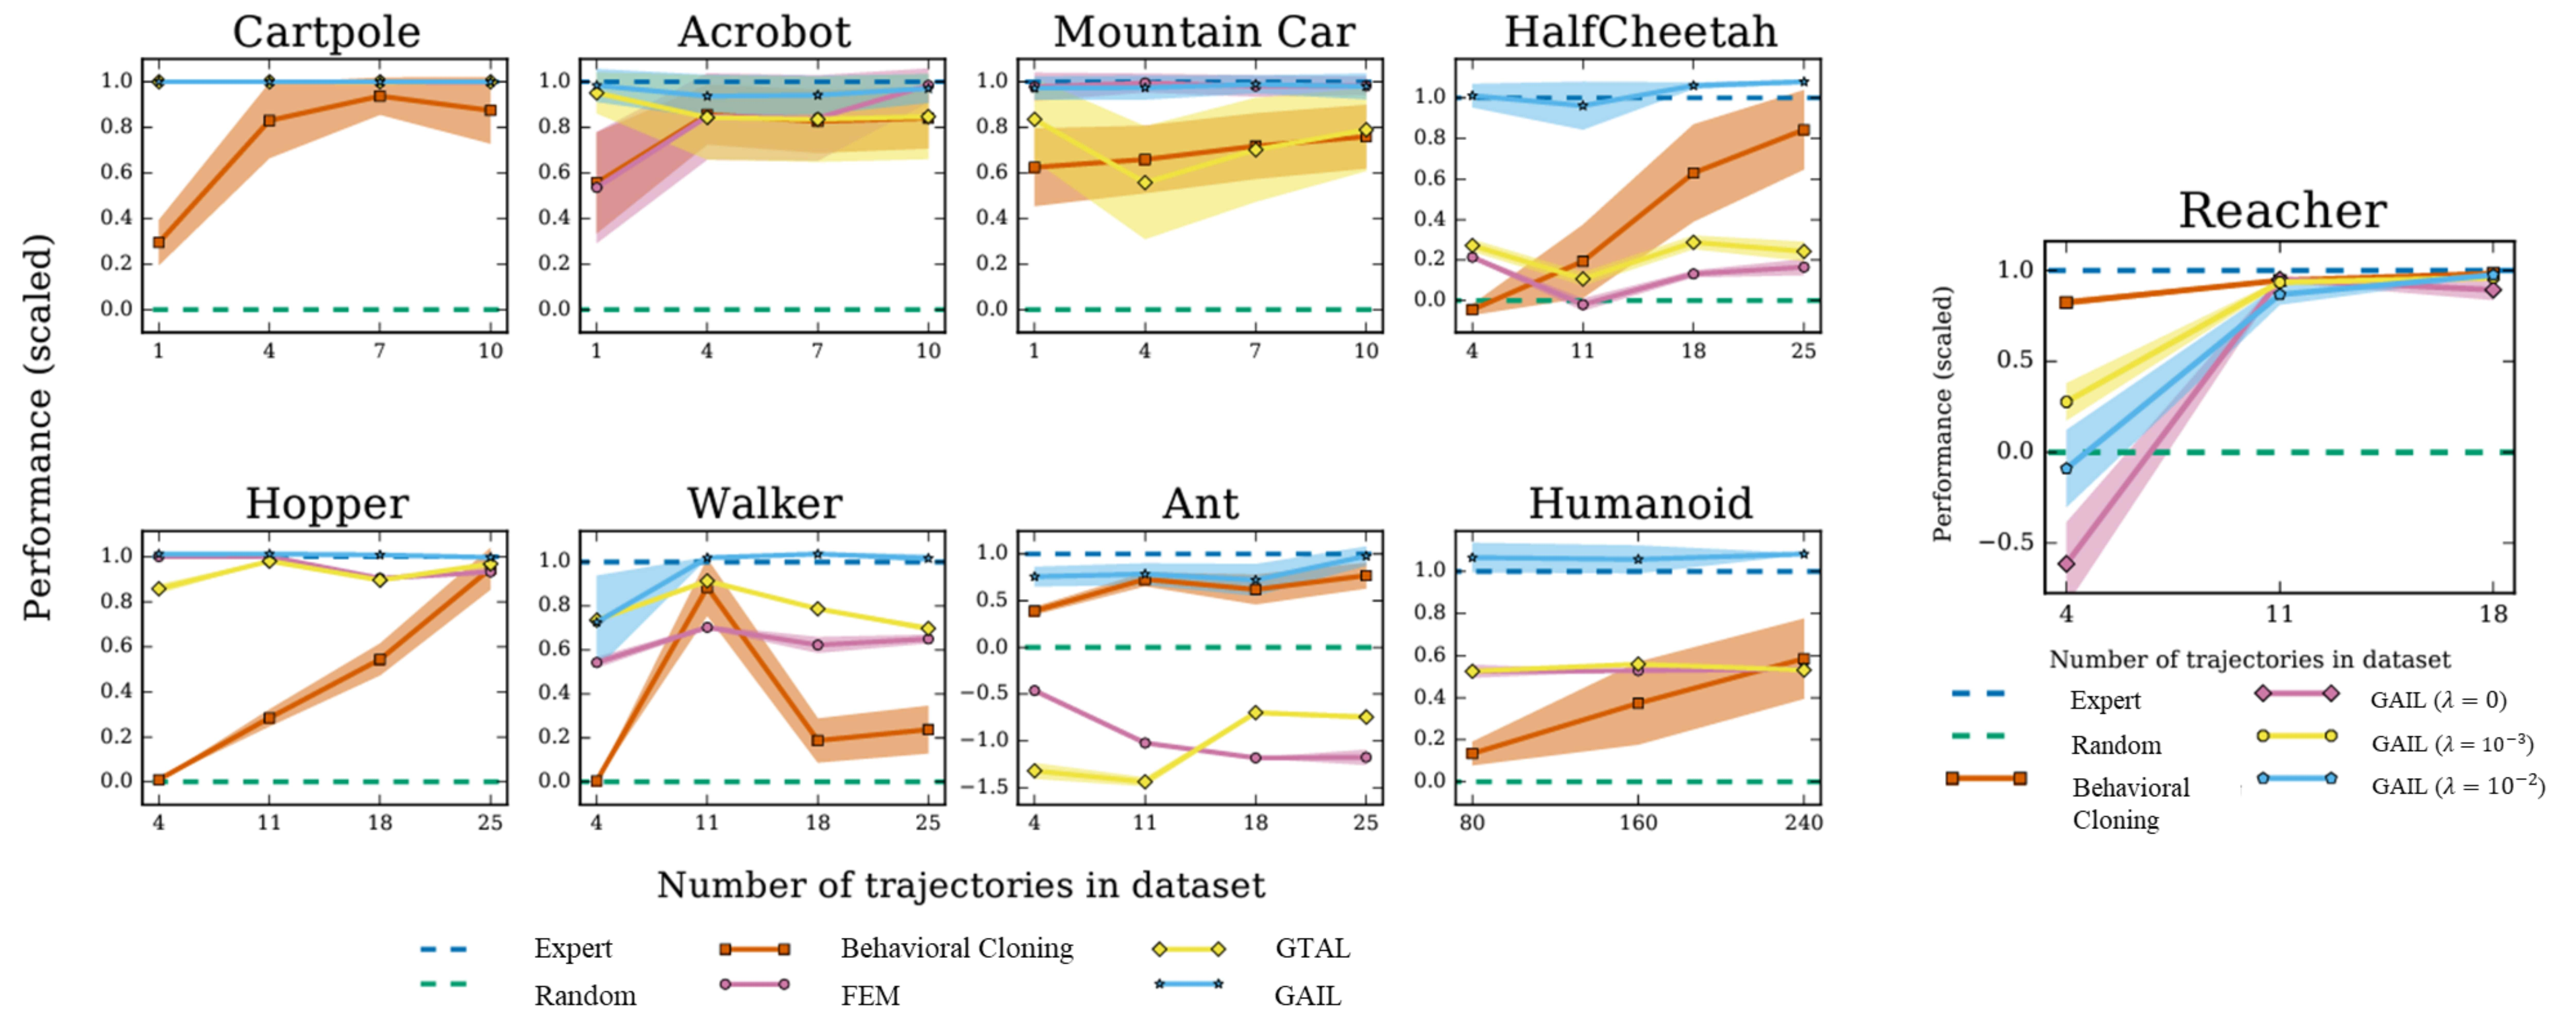
\includegraphics[width=\textwidth]{figures/images/gail_performance.png}
    \caption{The performance comparison proposed in \cite{ho2016gail} is presented here. The y-axis shows the scaled reward, where the expert's reward is set to 1 and the random baseline is set to 0. The IRL baselines FEM and GTAL refer to the IRL algorithm described in \cite{ho2016model}, but with different cost functions.}
    \label{fig:gail_performance}
    
\end{figure}




\begin{table}[t]
    \centering
    \tiny
    \selectfont
    \caption{Observation and Action space for the tasks used in~\cite{ho2016gail}}
    \label{table:gail_tasks}
    \resizebox{\linewidth}{!}{%
    \begin{tabular}{|c|c|c|} 
    \hline
    \textbf{Task} & \textbf{Observation space} & \textbf{Action space} \\ 
    \hhline{|===|}
    Cartpole & 4 (continuous) & 2 (discrete) \\ 
    \hline
    Acrobot & 4 (continuous) & 3 (discrete) \\ 
    \hline
    Mountain Car & 2 (continuous) & 3 (discrete) \\ 
    \hline
    Reacher & 11 (continuous) & 2 (continuous) \\ 
    \hline
    HalfCheetah & 17 (continuous) & 6 (continuous) \\ 
    \hline
    Hopper & 11 (continuous) & 3 (continuous) \\ 
    \hline
    Walker & 17 (continuous) & 6 (continuous) \\ 
    \hline
    Ant & 111 (continuous) & 8 (continuous) \\ 
    \hline
    Humanoid & 376 (continuous) & 17 (continuous) \\
    \hline
    \end{tabular}
    }
    \end{table} 

The observation and control spaces for these tasks are detailed in Table \ref{table:gail_tasks}, and the performance results are shown in Figure \ref{fig:gail_performance}. From these results, it is evident that the GAIL algorithm overcomes classic IRL algorithms in terms of both pure reward and sample efficiency. Consequently, subsequent research has focused on improving the algorithm's efficiency in terms of environment interaction. This has been achieved by replacing the model-free, on-policy TRPO algorithm with an off-policy RL algorithm, as seen in \cite{kostrikov2018discriminator}, or by modifying the reward function input to the RL algorithm \cite{fu2018airl,ghasemipour2020divergence_minimization_perspective}.

However, as noted in Table \ref{table:gail_tasks}, the tested tasks are characterized by low-dimensional state spaces. More recent research \cite{liu2018imitation_from_observation,reddy2019sqil,zolna2021task_relevant_ail,rafailov2021visual_ail} has focused on testing the GAIL algorithms in high-dimensional state spaces, where the input is an image. Specifically, with respect to the Adversarial Imitation Learning setting, works of interest are \cite{zolna2021task_relevant_ail,rafailov2021visual_ail}. 

In \cite{zolna2021task_relevant_ail}, the authors focused on solving the \textbf{casual confusion} problem. This problem occurs when the discriminator, during the learning process, focuses on task-irrelevant features between expert and policy generated transitions, for example a difference in the expert and agent embodiment like the gripper, this causes the rewards to become uninformative. To reduce the casual-confusion problem, in \cite{zolna2021task_relevant_ail} two elements have been proposed: 
\begin{enumerate}[label=\arabic*.]
    \item A \textit{regularization term}, with the aim to make the discriminator \textbf{unable} to distinguish between constraining sets $I_{E}$ and $I_{A}$. These sets are composed of expert and agent observations, such that a sample can belong either to $I_{E}$ or $I_{A}$, based on spurious features (e.g., a different gripper color);
    \item An \textit{early-stopping policy} called Actor Early-Stopping \\ (AES), that restarts the episode if the discriminator score at the current step exceeds the median score of the episode so far for $T_{patience}$ consecutive steps.
\end{enumerate} 

To prevent the discriminator from focusing on task irrelevant features, the authors proposed a regularization term based on the constraining-set accuracy defined in Formula \ref{eq:trail}. The idea is that if the discriminator achieves an accuracy greater than $\frac{1}{2}$ on the constraining set, the maximized adversarial cost function should be inverted, as shown in Formula \ref{eq:trail_discriminator}.

\begin{equation}
\label{eq:trail}
\textit{accuracy}(I_{E}, I_{A}) = \frac{1}{2} \ \mathbb{E}_{s \in I_{E}} \left[ \mathbf{1}_{D_{\omega} \geq  \frac{1}{2}}\right] + \frac{1}{2} \ \mathbb{E}_{s \in I_{A}} \left[ \mathbf{1}_{D_{\omega} <  \frac{1}{2}}\right] 
\end{equation}
\begin{equation}
    \label{eq:trail_discriminator}
    \begin{aligned}
        \mathcal{L}_\psi\left(s_E, s_A, \hat{s}_E, \hat{s}_A\right) 
        &= G_\psi\left(s_E, s_A\right) \\
        &\quad - \mathbf{1}_{\text {accuracy }\left(\hat{s}_E, \hat{s}_A\right) \geq \frac{1}{2}} G_\psi\left(\hat{s}_E, \hat{s}_A\right), \\ \\
        \text{where} \ \ G_\psi\left(s_E, s_A\right) 
        &= \sum_{i=1}^N \log D_\psi\left(s_E^{(i)}\right) \\
        &\quad + \log \left[1 - D_\psi\left(s_A^{(i)}\right)\right]
    \end{aligned}
\end{equation}
\begin{figure}[t]
    \centering
    \begin{subfigure}[b]{0.6\textwidth}
        \centering
        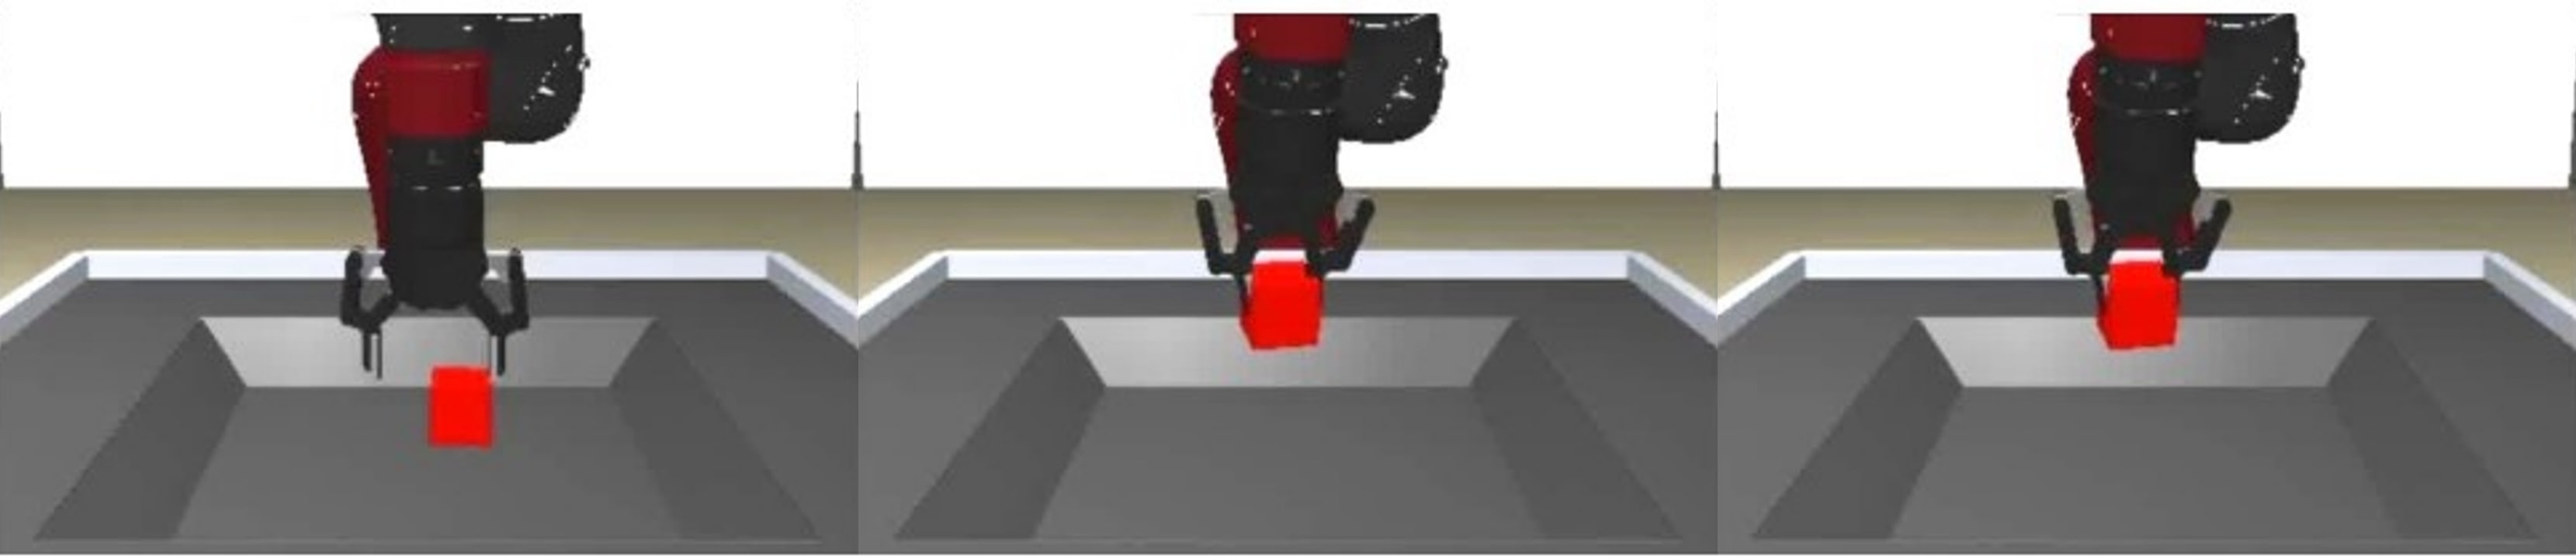
\includegraphics[width=\textwidth]{figures/images/trail/block_lifting.jpg}
        \caption{Lifting task.}
    \end{subfigure}
    \vfill
    \begin{subfigure}[b]{0.6\textwidth}
        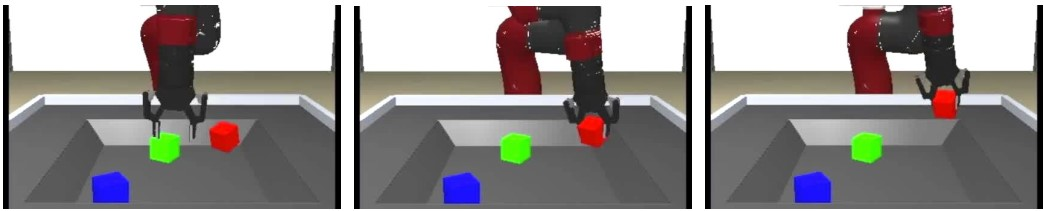
\includegraphics[width=\textwidth]{figures/images/trail/block_lifting_with_distractors}
        \caption{Lifting with distractors task.}
    \end{subfigure}
    \vfill
    \begin{subfigure}[b]{0.6\textwidth}
        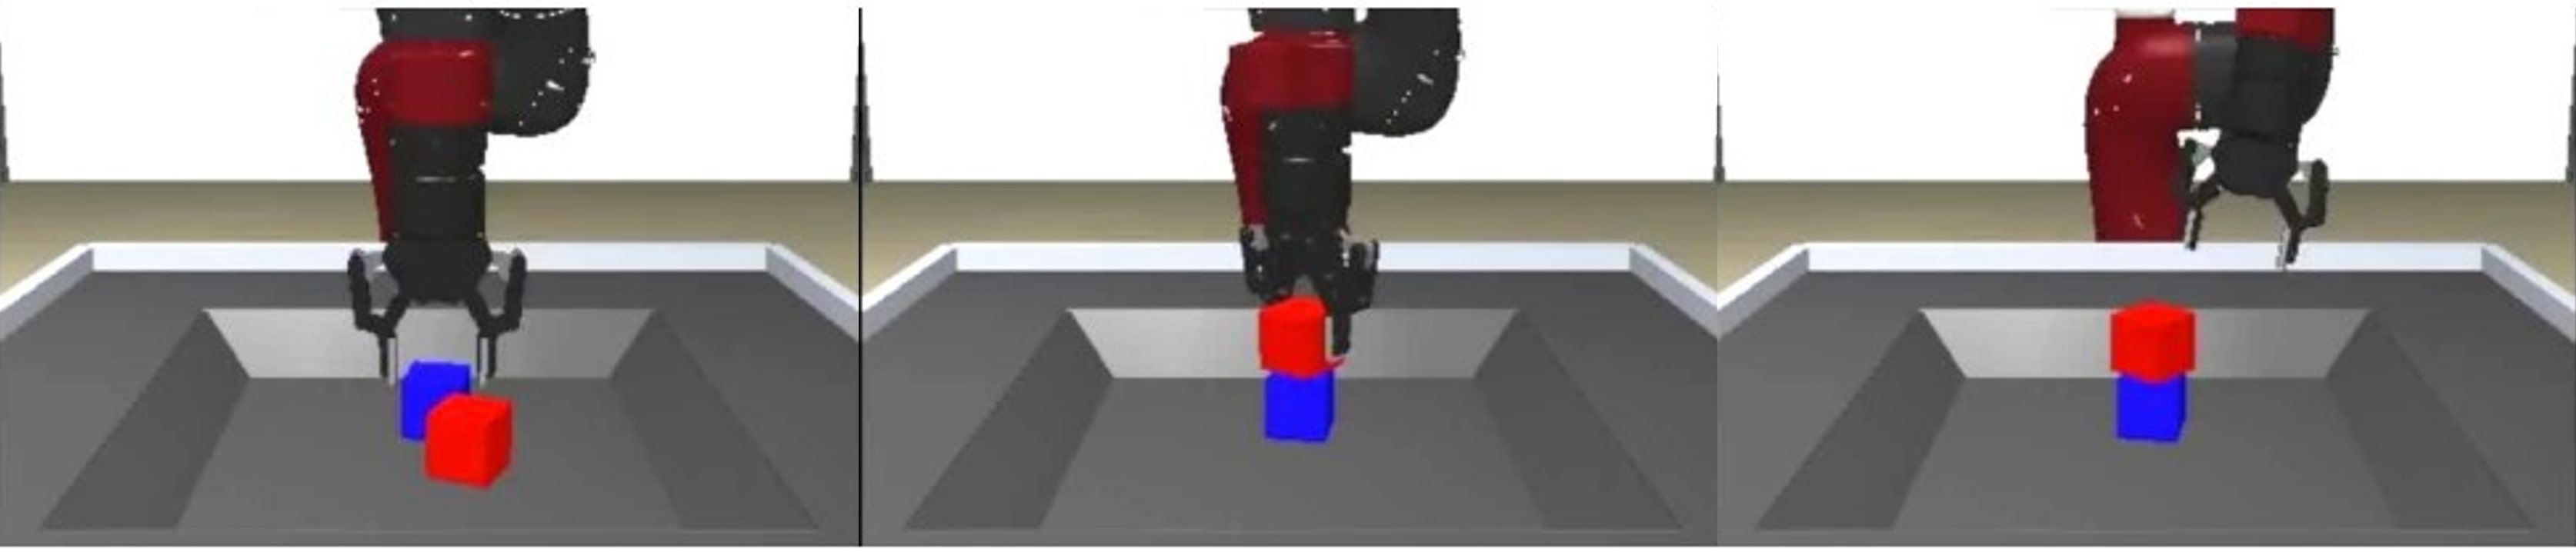
\includegraphics[width=\textwidth]{figures/images/trail/block_stacking}
        \caption{Block Stacking task.}
    \end{subfigure}
    \vfill
    \begin{subfigure}[b]{0.6\textwidth}
        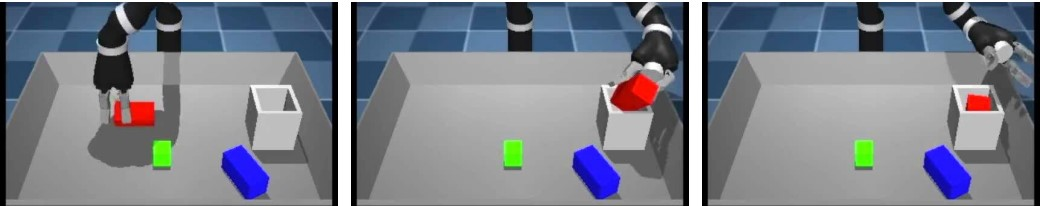
\includegraphics[width=\textwidth]{figures/images/trail/block_insertion_with_distractors}
        \caption{Block Insertion with distractors task.}
    \end{subfigure}
    \caption{Tasks solved in~\cite{zolna2021task_relevant_ail}.}
    \label{fig:trail_tasks}
\end{figure}

The proposed system was tested on 4 tasks (Figure \ref{fig:trail_tasks}), with the agent trained on each single task, according to the \textit{Distributed Distributional Deterministic Policy Gradients} (D4PG) \cite{barth2018d4pg} RL algorithm, with reward-function $R(s_{t}) = - \log(1-D_{\omega}(s_{t}))$. Experimental results have shown how the proposed system overcomes the GAIL \cite{ho2016gail} baseline, both in setting with spurious features and without spurious features (Figure \ref{fig:trail_results}).
\begin{figure}[t]
    \centering
    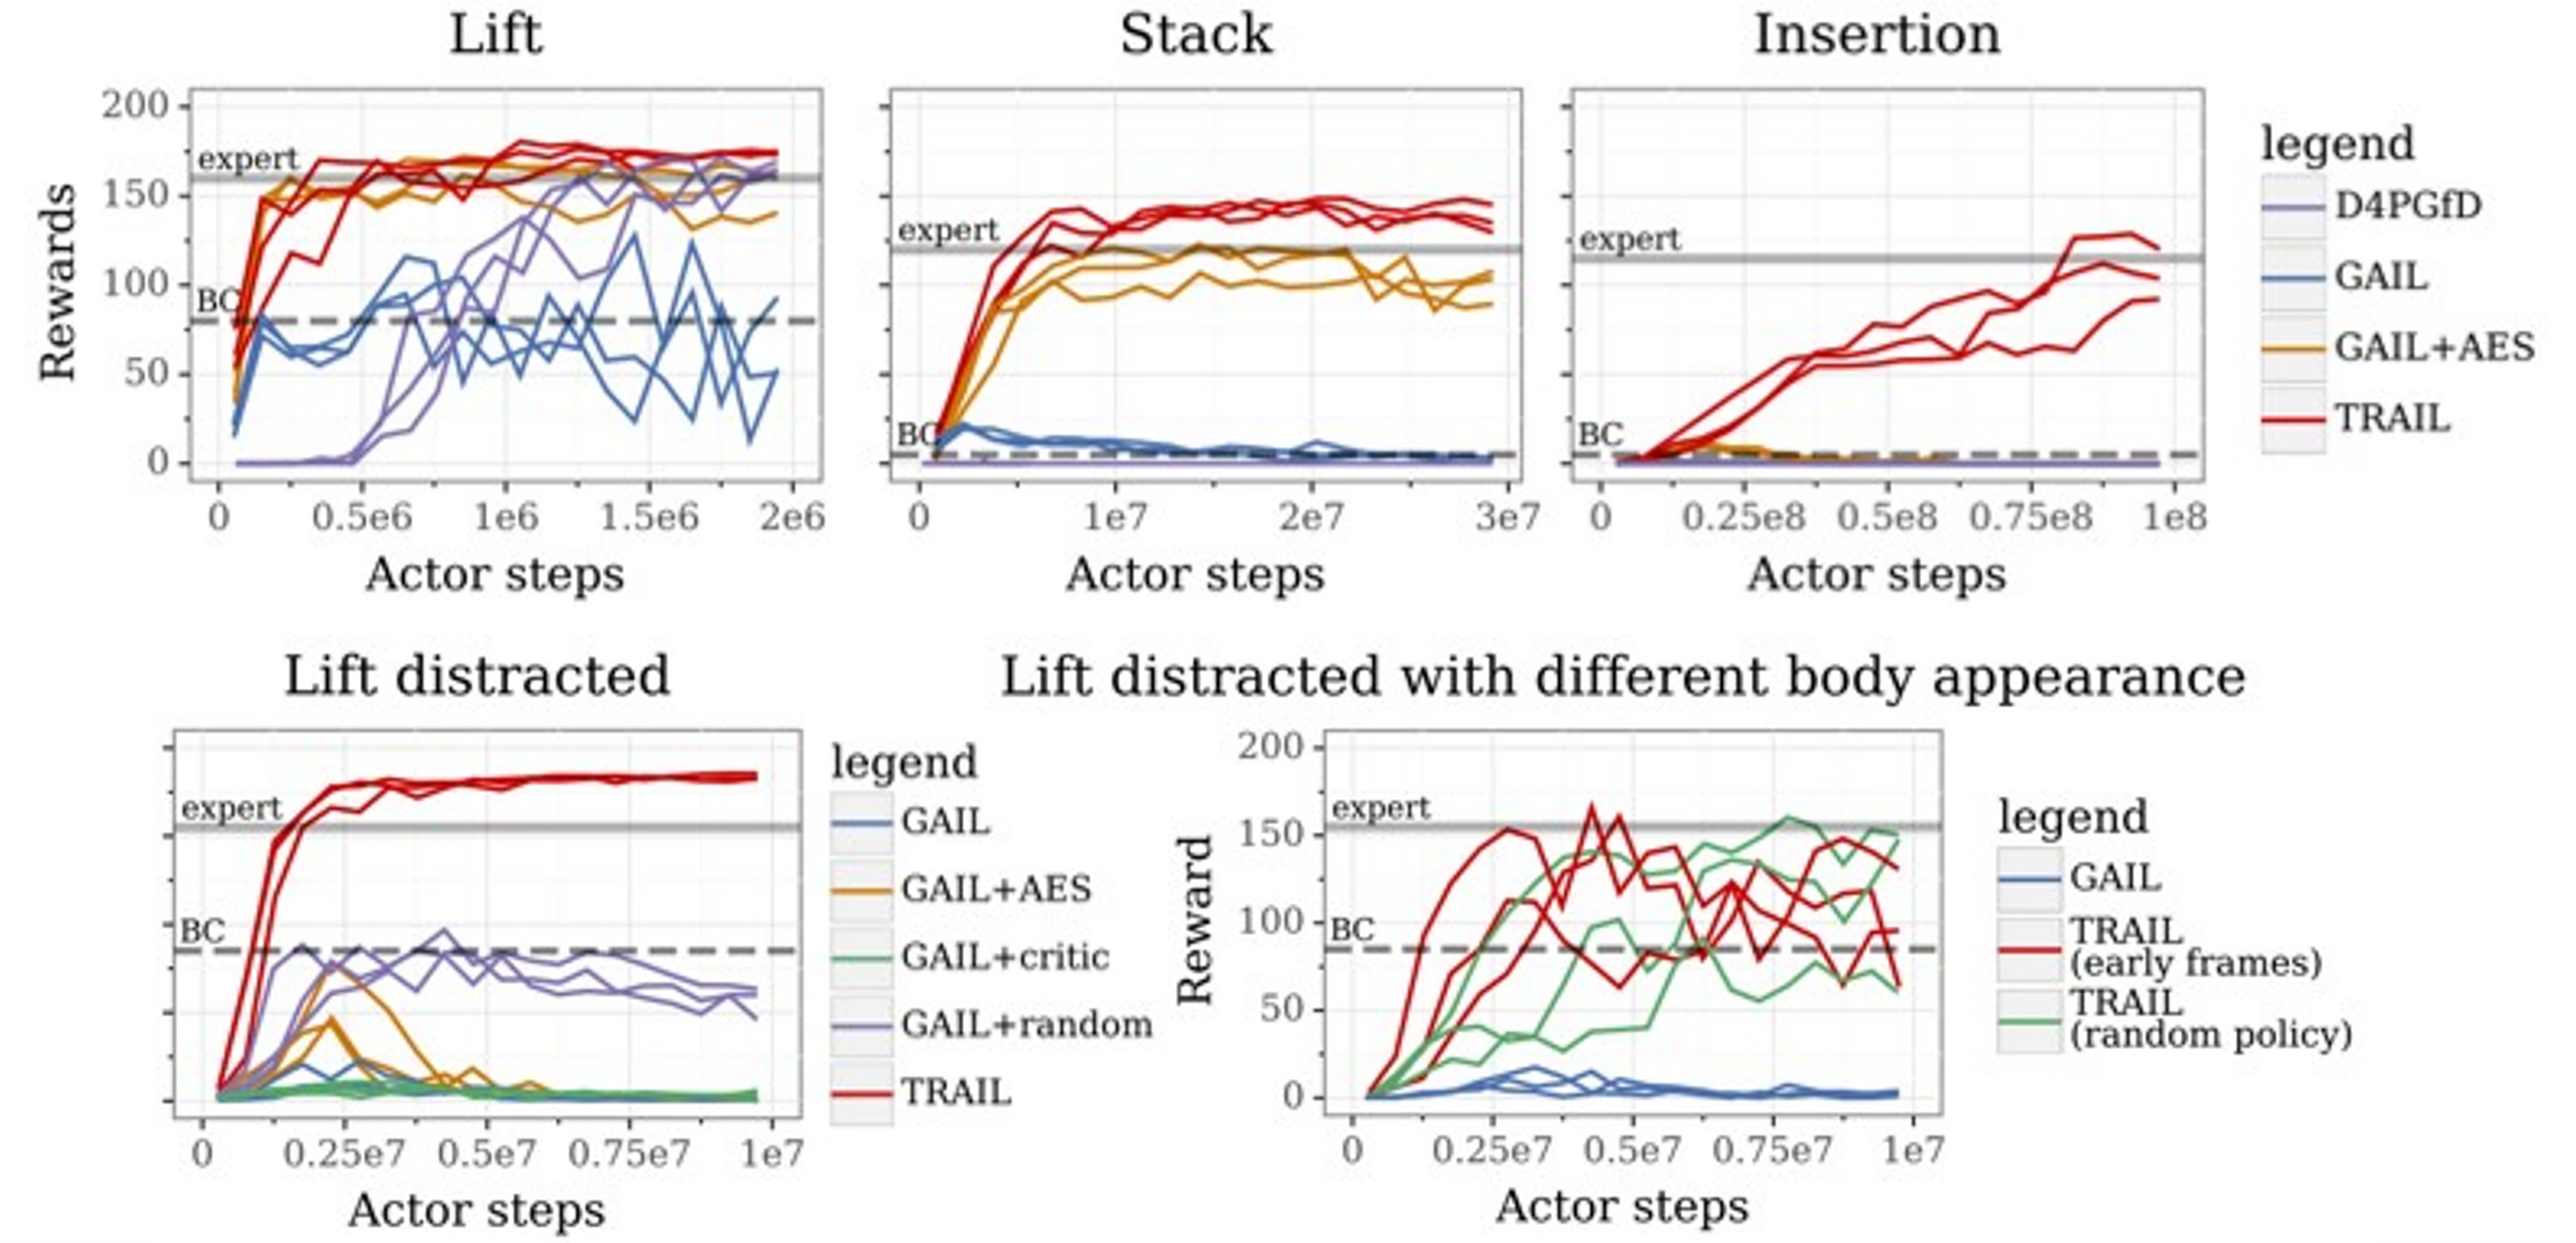
\includegraphics[width=0.8\textwidth]{Figures/images/trail/trail_results.png}
    \caption{Experimental results on tasks without and with spurious features~\cite{zolna2021task_relevant_ail}}    
   \label{fig:trail_results}
\end{figure}




The authors of \cite{rafailov2021visual_ail} proposed a more data-efficient Adversarial Imitation Learning method. They leveraged a model-based approach within a high-dimensional state space. Instead of generating a dynamic model in the image space, i.e., training a generative model to produce the next image based on the current image and the performed action.Their method encodes observations defined in the image space into a corresponding latent space characterized by vectors of smaller dimensions. Then, they learn a dynamic model in that space, training a generative model to produce the next embedding based on the current encoded observation and the performed action. The proposed learning procedure is based on three main steps:
\begin{enumerate}[label=\arabic*.]
    \item Learn the \textit{Latent Dynamic Model}, $(\hat{\mathcal{U}}_{\beta},\hat{\mathcal{T}}_{\beta}, q_{beta})$, by maximizing the Evidence Lower Bound (Formula \ref{formula:elbo}), where $\hat{\mathcal{U}}_{\beta}$ is the decoder, $q_{beta}$ is the encoder, and $\hat{\mathcal{T}}_{\beta}$ is the transition model;
    \item Train a \textit{discriminator}, $D_{\theta}$, by minimizing the Adversarial Loss function (Formula \ref{formula:discriminator});
    \item Train a \textit{policy} $\pi^{L}_{\theta}$, by maximizing the Value function (Formula \ref{formula:value_function}).
\end{enumerate}
\begin{align}
    \label{formula:elbo}
    \underset{\beta}{\max} \ & \mathbb{E}_{q_{\beta}} \left[ \sum_{t} \log(\mathcal{\hat{U}}_{\beta}(s_{t}|z_{t})) \right. \nonumber \\
    &\left. + \mathbb{D}_{KL}(q_{\beta}(z_{t}|s_{t},z_{t-1},a_{t-1})|| \mathcal{\hat{T}}_{\beta}(z_{t}|z_{t-1},a_{t-1})) \right]
\end{align}

\begin{align}
    \label{formula:discriminator}
    \underset{\theta}{\min} \ & \mathbb{E}_{(z,a) \sim \rho^{E}(z,a)} \left[ -\log(D_{\theta}(z,a)) \right] \nonumber \\
    & + \mathbb{E}_{(z,a) \sim \rho^{\pi^{L}}_{\hat{\mathcal{T}}}} \left[ -\log(1 - D_{\theta}(z,a)) \right]
\end{align}

\begin{align}
    \label{formula:value_function}
    \underset{\pi^{L}_{\theta}}{\max} \ V^{K}_{\theta,\beta}(z_{t}) 
    &= \underset{\pi^{L}_{\theta}}{\max} \ \mathbb{E}_{\pi^{L}_{\theta}, \mathcal{\hat{T}}_{\beta}} \left[ \sum_{\tau = t}^{t+K-1} \gamma^{\tau-t} \log(D_{\theta}(z_{\tau}^{\pi^{L}_{\theta}}, a_{\tau}^{\pi^{L}_{\theta}})) \right. \nonumber \\
    &\left. + \gamma^{K}V_{\beta}(z_{t+K}^{\pi^{L}_{\theta}}) \right]
\end{align}

    
With this learning setting the proposed system outperforms previous works such as \cite{reddy2019sqil,kostrikov2018discriminator} both in terms of \textbf{data efficiency} and \textbf{overall performance}, on a set of continous control tasks.
% \begin{align}
    \label{formula:elbo}
    \underset{\beta}{\max} \ & \mathbb{E}_{q_{\beta}} \left[ \sum_{t} \log(\mathcal{\hat{U}}_{\beta}(s_{t}|z_{t})) \right. \nonumber \\
    &\left. + \mathbb{D}_{KL}(q_{\beta}(z_{t}|s_{t},z_{t-1},a_{t-1})|| \mathcal{\hat{T}}_{\beta}(z_{t}|z_{t-1},a_{t-1})) \right]
\end{align}

\begin{align}
    \label{formula:discriminator}
    \underset{\theta}{\min} \ & \mathbb{E}_{(z,a) \sim \rho^{E}(z,a)} \left[ -\log(D_{\theta}(z,a)) \right] \nonumber \\
    & + \mathbb{E}_{(z,a) \sim \rho^{\pi^{L}}_{\hat{\mathcal{T}}}} \left[ -\log(1 - D_{\theta}(z,a)) \right]
\end{align}

\begin{align}
    \label{formula:value_function}
    \underset{\pi^{L}_{\theta}}{\max} \ V^{K}_{\theta,\beta}(z_{t}) 
    &= \underset{\pi^{L}_{\theta}}{\max} \ \mathbb{E}_{\pi^{L}_{\theta}, \mathcal{\hat{T}}_{\beta}} \left[ \sum_{\tau = t}^{t+K-1} \gamma^{\tau-t} \log(D_{\theta}(z_{\tau}^{\pi^{L}_{\theta}}, a_{\tau}^{\pi^{L}_{\theta}})) \right. \nonumber \\
    &\left. + \gamma^{K}V_{\beta}(z_{t+K}^{\pi^{L}_{\theta}}) \right]
\end{align}

    

Generally speaking, the Generative Adversarial Imitation Learning has shown very promising performance in simulated control tasks and simulated robot manipulation tasks, even in complex high-dimensional state-space. However, it is not so clear, how these methods could perform in real-world robotic manipulation tasks, in terms of data-efficiency, generalization capability, and safety during real-world interactions. 